%#########################################

% author: S. Parisa Daj.
% email: s.dajkhosh@memphis.edu
% University of Memphis
% Sep 2021

%#########################################

\documentclass[12pt,oneside,geqno]{article}

\addtolength{\textheight}{120pt}
\oddsidemargin=-10pt
\topmargin=-.5in
\textwidth=6.5in
\pagestyle{empty}

% ######################## 	Packages
\usepackage{amssymb,latexsym,amsmath,amsthm}
\usepackage{amsfonts,raWFonts}
\usepackage{thmtools}
\usepackage{systeme}
\usepackage{mathtools}
\usepackage[usenames,dvipsnames]{color}
\usepackage{xcolor}
\usepackage{xfrac}
\usepackage{hyperref}
\usepackage[utf8]{inputenc}
\usepackage{enumerate}



\usepackage{listings}
\usepackage{xcolor}

\usepackage{graphicx}
\usepackage{caption}
\usepackage{subcaption}

% ######################## 	Colors
\definecolor{codegreen}{rgb}{0,0.6,0}
\definecolor{codegray}{rgb}{0.5,0.5,0.5}
\definecolor{codepurple}{rgb}{0.58,0,0.82}
\definecolor{backcolour}{rgb}{0.97,0.97,0.95}

% ######################## 	Style
\lstdefinestyle{mystyle}{
	backgroundcolor=\color{backcolour},   
	commentstyle=\color{codegreen},
	keywordstyle=\color{magenta},
	numberstyle=\tiny\color{codegray},
	stringstyle=\color{codepurple},
	basicstyle=\ttfamily\footnotesize,
	breakatwhitespace=false,         
	breaklines=true,                 
	captionpos=b,                    
	keepspaces=true,                 
	numbers=left,                    
	numbersep=5pt,                  
	showspaces=false,                
	showstringspaces=false,
	showtabs=false,                  
	tabsize=2
}

\lstset{style=mystyle}

\declaretheoremstyle[
headfont=\color{blue}\normalfont\bfseries,
notefont=\bfseries, 
notebraces={}{},
%bodyfont=\color{red}\normalfont\itshape,
bodyfont=\normalfont,%\itshape,
%headformat=\NUMBER.~\NAME\NOTE
headformat=\NAME\NOTE
]{colorejercicio}

\declaretheorem[
%numbered=no,
style=colorejercicio,
name=Problem
]{Problem}

% ######################## 	Document
\begin{document}
	
	\begin{center}
		{\LARGE EECE 8740-Neural Networks HW \#3}% Title
		\vspace*{1\baselineskip}   
		
		\scshape % Small caps
		\color{red}{(Solutions)}\\
		%  
		\vspace*{1\baselineskip}
		\color{black}University of Memphis\\[\baselineskip]
		%
		\vspace*{5\baselineskip} 
		
		Written by \\[\baselineskip]
		{\Large S. Parisa Daj.\par U00743495} \\
		(s.dajkhosh@memphis.edu)\\
		
		\vspace*{1\baselineskip}
		\today
	\end{center}
	%
	\clearpage
	
	
	\section{Introduction}
	The goal of this assignment is to implement either a ResNet32 or a ResNet50 model. The data used for this task is the Tiny ImageNet dataset which includes 100000 RGB images of 200 different classes. Each image is 64x64 square-sized. In the first question, we are evaluating the said dataset on the ResNet50 model. ResNet50 is a residual neural network designed and pre-trained on millions of images in 1000 various classes. This model is 50 layers deep. After the evaluation, the model will be fine-tuned with the new images. The next step is to ensemble and compare the result of the two previous layers with the best model trained in assignment 2. It is expected to have the highest accuracy from the second task because we fine-tune a very powerful pre-trained model. 
	
	\begin{table}[]
		\resizebox{\textwidth}{!}{\begin{tabular}{llll}
				\hline
				Layer (type)                                           & Output Shape                              & Param \#                     & Connected to                                              \\ \hline
				\multicolumn{1}{|l|}{input\_2 (InputLayer)}            & \multicolumn{1}{l|}{(None, 224, 224, 3)}  & \multicolumn{1}{l|}{0}       & \multicolumn{1}{l|}{}                                     \\ \hline
				\multicolumn{1}{|l|}{conv1\_pad (ZeroPadding2D)}       & \multicolumn{1}{l|}{(None, 230, 230, 3)}  & \multicolumn{1}{l|}{0}       & \multicolumn{1}{l|}{input\_2{[}0{]}{[}0{]}}               \\ \hline
				\multicolumn{1}{|l|}{conv1\_conv (Conv2D)}             & \multicolumn{1}{l|}{(None, 112, 112, 64)} & \multicolumn{1}{l|}{9472}    & \multicolumn{1}{l|}{conv1\_pad{[}0{]}{[}0{]}}             \\ \hline
				\multicolumn{1}{|l|}{pool1\_pad (ZeroPadding2D)}       & \multicolumn{1}{l|}{(None, 114, 114, 64)} & \multicolumn{1}{l|}{0}       & \multicolumn{1}{l|}{conv1\_relu{[}0{]}{[}0{]}}            \\ \hline
				\multicolumn{1}{|l|}{pool1\_pool (MaxPooling2D)}       & \multicolumn{1}{l|}{(None, 56, 56, 64)}   & \multicolumn{1}{l|}{0}       & \multicolumn{1}{l|}{pool1\_pad{[}0{]}{[}0{]}}             \\ \hline
				\multicolumn{1}{|l|}{conv2\_block1\_1\_conv (Conv2D)}  & \multicolumn{1}{l|}{(None, 56, 56, 64)}   & \multicolumn{1}{l|}{4160}    & \multicolumn{1}{l|}{pool1\_pool{[}0{]}{[}0{]}}            \\ \hline
				\multicolumn{1}{|l|}{conv2\_block1\_2\_conv (Conv2D)}  & \multicolumn{1}{l|}{(None, 56, 56, 64)}   & \multicolumn{1}{l|}{36928}   & \multicolumn{1}{l|}{conv2\_block1\_1\_relu{[}0{]}{[}0{]}} \\ \hline
				\multicolumn{1}{|l|}{conv2\_block1\_0\_conv (Conv2D)}  & \multicolumn{1}{l|}{(None, 56, 56, 256)}  & \multicolumn{1}{l|}{16640}   & \multicolumn{1}{l|}{pool1\_pool{[}0{]}{[}0{]}}            \\ \hline
				\multicolumn{1}{|l|}{conv2\_block1\_3\_conv (Conv2D)}  & \multicolumn{1}{l|}{(None, 56, 56, 256)}  & \multicolumn{1}{l|}{16640}   & \multicolumn{1}{l|}{conv2\_block1\_2\_relu{[}0{]}{[}0{]}} \\ \hline
				\multicolumn{1}{|l|}{conv2\_block2\_1\_conv (Conv2D)}  & \multicolumn{1}{l|}{(None, 56, 56, 64)}   & \multicolumn{1}{l|}{16448}   & \multicolumn{1}{l|}{conv2\_block1\_out{[}0{]}{[}0{]}}     \\ \hline
				\multicolumn{1}{|l|}{conv2\_block2\_2\_conv (Conv2D)}  & \multicolumn{1}{l|}{(None, 56, 56, 64)}   & \multicolumn{1}{l|}{36928}   & \multicolumn{1}{l|}{conv2\_block2\_1\_relu{[}0{]}{[}0{]}} \\ \hline
				\multicolumn{1}{|l|}{conv2\_block2\_3\_conv (Conv2D)}  & \multicolumn{1}{l|}{(None, 56, 56, 256)}  & \multicolumn{1}{l|}{16640}   & \multicolumn{1}{l|}{conv2\_block2\_2\_relu{[}0{]}{[}0{]}} \\ \hline
				\multicolumn{1}{|l|}{conv2\_block3\_1\_conv (Conv2D)}  & \multicolumn{1}{l|}{(None, 56, 56, 64)}   & \multicolumn{1}{l|}{16448}   & \multicolumn{1}{l|}{conv2\_block2\_out{[}0{]}{[}0{]}}     \\ \hline
				\multicolumn{1}{|l|}{conv2\_block3\_2\_conv (Conv2D)}  & \multicolumn{1}{l|}{(None, 56, 56, 64)}   & \multicolumn{1}{l|}{36928}   & \multicolumn{1}{l|}{conv2\_block3\_1\_relu{[}0{]}{[}0{]}} \\ \hline
				\multicolumn{1}{|l|}{conv2\_block3\_3\_conv (Conv2D)}  & \multicolumn{1}{l|}{(None, 56, 56, 256)}  & \multicolumn{1}{l|}{16640}   & \multicolumn{1}{l|}{conv2\_block3\_2\_relu{[}0{]}{[}0{]}} \\ \hline
				\multicolumn{1}{|l|}{conv3\_block1\_1\_conv (Conv2D)}  & \multicolumn{1}{l|}{(None, 28, 28, 128)}  & \multicolumn{1}{l|}{32896}   & \multicolumn{1}{l|}{conv2\_block3\_out{[}0{]}{[}0{]}}     \\ \hline
				\multicolumn{1}{|l|}{conv3\_block1\_2\_conv (Conv2D)}  & \multicolumn{1}{l|}{(None, 28, 28, 128)}  & \multicolumn{1}{l|}{147584}  & \multicolumn{1}{l|}{conv3\_block1\_1\_relu{[}0{]}{[}0{]}} \\ \hline
				\multicolumn{1}{|l|}{conv3\_block1\_0\_conv (Conv2D)}  & \multicolumn{1}{l|}{(None, 28, 28, 512)}  & \multicolumn{1}{l|}{131584}  & \multicolumn{1}{l|}{conv2\_block3\_out{[}0{]}{[}0{]}}     \\ \hline
				\multicolumn{1}{|l|}{conv3\_block1\_3\_conv (Conv2D)}  & \multicolumn{1}{l|}{(None, 28, 28, 512)}  & \multicolumn{1}{l|}{66048}   & \multicolumn{1}{l|}{conv3\_block1\_2\_relu{[}0{]}{[}0{]}} \\ \hline
				\multicolumn{1}{|l|}{conv3\_block2\_1\_conv (Conv2D)}  & \multicolumn{1}{l|}{(None, 28, 28, 128)}  & \multicolumn{1}{l|}{65664}   & \multicolumn{1}{l|}{conv3\_block1\_out{[}0{]}{[}0{]}}     \\ \hline
				\multicolumn{1}{|l|}{conv3\_block2\_2\_conv (Conv2D)}  & \multicolumn{1}{l|}{(None, 28, 28, 128)}  & \multicolumn{1}{l|}{147584}  & \multicolumn{1}{l|}{conv3\_block2\_1\_relu{[}0{]}{[}0{]}} \\ \hline
				\multicolumn{1}{|l|}{conv3\_block2\_3\_conv (Conv2D)}  & \multicolumn{1}{l|}{(None, 28, 28, 512)}  & \multicolumn{1}{l|}{66048}   & \multicolumn{1}{l|}{conv3\_block2\_2\_relu{[}0{]}{[}0{]}} \\ \hline
				\multicolumn{1}{|l|}{conv3\_block3\_1\_conv (Conv2D)}  & \multicolumn{1}{l|}{(None, 28, 28, 128)}  & \multicolumn{1}{l|}{65664}   & \multicolumn{1}{l|}{conv3\_block2\_out{[}0{]}{[}0{]}}     \\ \hline
				\multicolumn{1}{|l|}{conv3\_block3\_2\_conv (Conv2D)}  & \multicolumn{1}{l|}{(None, 28, 28, 128)}  & \multicolumn{1}{l|}{147584}  & \multicolumn{1}{l|}{conv3\_block3\_1\_relu{[}0{]}{[}0{]}} \\ \hline
				\multicolumn{1}{|l|}{conv3\_block3\_3\_conv (Conv2D)}  & \multicolumn{1}{l|}{(None, 28, 28, 512)}  & \multicolumn{1}{l|}{66048}   & \multicolumn{1}{l|}{conv3\_block3\_2\_relu{[}0{]}{[}0{]}} \\ \hline
				\multicolumn{1}{|l|}{conv3\_block4\_1\_conv (Conv2D)}  & \multicolumn{1}{l|}{(None, 28, 28, 128)}  & \multicolumn{1}{l|}{65664}   & \multicolumn{1}{l|}{conv3\_block3\_out{[}0{]}{[}0{]}}     \\ \hline
				\multicolumn{1}{|l|}{conv3\_block4\_2\_conv (Conv2D)}  & \multicolumn{1}{l|}{(None, 28, 28, 128)}  & \multicolumn{1}{l|}{147584}  & \multicolumn{1}{l|}{conv3\_block4\_1\_relu{[}0{]}{[}0{]}} \\ \hline
				\multicolumn{1}{|l|}{conv3\_block4\_3\_conv (Conv2D)}  & \multicolumn{1}{l|}{(None, 28, 28, 512)}  & \multicolumn{1}{l|}{66048}   & \multicolumn{1}{l|}{conv3\_block4\_2\_relu{[}0{]}{[}0{]}} \\ \hline
				\multicolumn{1}{|l|}{conv4\_block1\_1\_conv (Conv2D)}  & \multicolumn{1}{l|}{(None, 14, 14, 256)}  & \multicolumn{1}{l|}{131328}  & \multicolumn{1}{l|}{conv3\_block4\_out{[}0{]}{[}0{]}}     \\ \hline
				\multicolumn{1}{|l|}{conv4\_block1\_2\_conv (Conv2D)}  & \multicolumn{1}{l|}{(None, 14, 14, 256)}  & \multicolumn{1}{l|}{590080}  & \multicolumn{1}{l|}{conv4\_block1\_1\_relu{[}0{]}{[}0{]}} \\ \hline
				\multicolumn{1}{|l|}{conv4\_block1\_0\_conv (Conv2D)}  & \multicolumn{1}{l|}{(None, 14, 14, 1024)} & \multicolumn{1}{l|}{525312}  & \multicolumn{1}{l|}{conv3\_block4\_out{[}0{]}{[}0{]}}     \\ \hline
				\multicolumn{1}{|l|}{conv4\_block1\_3\_conv (Conv2D)}  & \multicolumn{1}{l|}{(None, 14, 14, 1024)} & \multicolumn{1}{l|}{263168}  & \multicolumn{1}{l|}{conv4\_block1\_2\_relu{[}0{]}{[}0{]}} \\ \hline
				\multicolumn{1}{|l|}{conv4\_block2\_1\_conv (Conv2D)}  & \multicolumn{1}{l|}{(None, 14, 14, 256)}  & \multicolumn{1}{l|}{262400}  & \multicolumn{1}{l|}{conv4\_block1\_out{[}0{]}{[}0{]}}     \\ \hline
				\multicolumn{1}{|l|}{conv4\_block2\_2\_conv (Conv2D)}  & \multicolumn{1}{l|}{(None, 14, 14, 256)}  & \multicolumn{1}{l|}{590080}  & \multicolumn{1}{l|}{conv4\_block2\_1\_relu{[}0{]}{[}0{]}} \\ \hline
				\multicolumn{1}{|l|}{conv4\_block2\_3\_conv (Conv2D)}  & \multicolumn{1}{l|}{(None, 14, 14, 1024)} & \multicolumn{1}{l|}{263168}  & \multicolumn{1}{l|}{conv4\_block2\_2\_relu{[}0{]}{[}0{]}} \\ \hline
				\multicolumn{1}{|l|}{conv4\_block3\_1\_conv (Conv2D)}  & \multicolumn{1}{l|}{(None, 14, 14, 256)}  & \multicolumn{1}{l|}{262400}  & \multicolumn{1}{l|}{conv4\_block2\_out{[}0{]}{[}0{]}}     \\ \hline
				\multicolumn{1}{|l|}{conv4\_block3\_2\_conv (Conv2D)}  & \multicolumn{1}{l|}{(None, 14, 14, 256)}  & \multicolumn{1}{l|}{590080}  & \multicolumn{1}{l|}{conv4\_block3\_1\_relu{[}0{]}{[}0{]}} \\ \hline
				\multicolumn{1}{|l|}{conv4\_block3\_3\_conv (Conv2D)}  & \multicolumn{1}{l|}{(None, 14, 14, 1024)} & \multicolumn{1}{l|}{263168}  & \multicolumn{1}{l|}{conv4\_block3\_2\_relu{[}0{]}{[}0{]}} \\ \hline
				\multicolumn{1}{|l|}{conv4\_block4\_1\_conv (Conv2D)}  & \multicolumn{1}{l|}{(None, 14, 14, 256)}  & \multicolumn{1}{l|}{262400}  & \multicolumn{1}{l|}{conv4\_block3\_out{[}0{]}{[}0{]}}     \\ \hline
				\multicolumn{1}{|l|}{conv4\_block4\_2\_conv (Conv2D)}  & \multicolumn{1}{l|}{(None, 14, 14, 256)}  & \multicolumn{1}{l|}{590080}  & \multicolumn{1}{l|}{conv4\_block4\_1\_relu{[}0{]}{[}0{]}} \\ \hline
				\multicolumn{1}{|l|}{conv4\_block4\_3\_conv (Conv2D)}  & \multicolumn{1}{l|}{(None, 14, 14, 1024)} & \multicolumn{1}{l|}{263168}  & \multicolumn{1}{l|}{conv4\_block4\_2\_relu{[}0{]}{[}0{]}} \\ \hline
				\multicolumn{1}{|l|}{conv4\_block5\_1\_conv (Conv2D)}  & \multicolumn{1}{l|}{(None, 14, 14, 256)}  & \multicolumn{1}{l|}{262400}  & \multicolumn{1}{l|}{conv4\_block4\_out{[}0{]}{[}0{]}}     \\ \hline
				\multicolumn{1}{|l|}{conv4\_block5\_2\_conv (Conv2D)}  & \multicolumn{1}{l|}{(None, 14, 14, 256)}  & \multicolumn{1}{l|}{590080}  & \multicolumn{1}{l|}{conv4\_block5\_1\_relu{[}0{]}{[}0{]}} \\ \hline
				\multicolumn{1}{|l|}{conv4\_block5\_3\_conv (Conv2D)}  & \multicolumn{1}{l|}{(None, 14, 14, 1024)} & \multicolumn{1}{l|}{263168}  & \multicolumn{1}{l|}{conv4\_block5\_2\_relu{[}0{]}{[}0{]}} \\ \hline
				\multicolumn{1}{|l|}{conv4\_block6\_1\_conv (Conv2D)}  & \multicolumn{1}{l|}{(None, 14, 14, 256)}  & \multicolumn{1}{l|}{262400}  & \multicolumn{1}{l|}{conv4\_block5\_out{[}0{]}{[}0{]}}     \\ \hline
				\multicolumn{1}{|l|}{conv4\_block6\_2\_conv (Conv2D)}  & \multicolumn{1}{l|}{(None, 14, 14, 256)}  & \multicolumn{1}{l|}{590080}  & \multicolumn{1}{l|}{conv4\_block6\_1\_relu{[}0{]}{[}0{]}} \\ \hline
				\multicolumn{1}{|l|}{conv4\_block6\_3\_conv (Conv2D)}  & \multicolumn{1}{l|}{(None, 14, 14, 1024)} & \multicolumn{1}{l|}{263168}  & \multicolumn{1}{l|}{conv4\_block6\_2\_relu{[}0{]}{[}0{]}} \\ \hline
				\multicolumn{1}{|l|}{conv5\_block1\_1\_conv (Conv2D)}  & \multicolumn{1}{l|}{(None, 7, 7, 512)}    & \multicolumn{1}{l|}{524800}  & \multicolumn{1}{l|}{conv4\_block6\_out{[}0{]}{[}0{]}}     \\ \hline
				\multicolumn{1}{|l|}{conv5\_block1\_2\_conv (Conv2D)}  & \multicolumn{1}{l|}{(None, 7, 7, 512)}    & \multicolumn{1}{l|}{2359808} & \multicolumn{1}{l|}{conv5\_block1\_1\_relu{[}0{]}{[}0{]}} \\ \hline
				\multicolumn{1}{|l|}{conv5\_block1\_0\_conv (Conv2D)}  & \multicolumn{1}{l|}{(None, 7, 7, 2048)}   & \multicolumn{1}{l|}{2099200} & \multicolumn{1}{l|}{conv4\_block6\_out{[}0{]}{[}0{]}}     \\ \hline
				\multicolumn{1}{|l|}{conv5\_block1\_3\_conv (Conv2D)}  & \multicolumn{1}{l|}{(None, 7, 7, 2048)}   & \multicolumn{1}{l|}{1050624} & \multicolumn{1}{l|}{conv5\_block1\_2\_relu{[}0{]}{[}0{]}} \\ \hline
				\multicolumn{1}{|l|}{conv5\_block2\_1\_conv (Conv2D)}  & \multicolumn{1}{l|}{(None, 7, 7, 512)}    & \multicolumn{1}{l|}{1049088} & \multicolumn{1}{l|}{conv5\_block1\_out{[}0{]}{[}0{]}}     \\ \hline
				\multicolumn{1}{|l|}{conv5\_block2\_2\_conv (Conv2D)}  & \multicolumn{1}{l|}{(None, 7, 7, 512)}    & \multicolumn{1}{l|}{2359808} & \multicolumn{1}{l|}{conv5\_block2\_1\_relu{[}0{]}{[}0{]}} \\ \hline
				\multicolumn{1}{|l|}{conv5\_block2\_3\_conv (Conv2D)}  & \multicolumn{1}{l|}{(None, 7, 7, 2048)}   & \multicolumn{1}{l|}{1050624} & \multicolumn{1}{l|}{conv5\_block2\_2\_relu{[}0{]}{[}0{]}} \\ \hline
				\multicolumn{1}{|l|}{conv5\_block3\_1\_conv (Conv2D)}  & \multicolumn{1}{l|}{(None, 7, 7, 512)}    & \multicolumn{1}{l|}{1049088} & \multicolumn{1}{l|}{conv5\_block2\_out{[}0{]}{[}0{]}}     \\ \hline
				\multicolumn{1}{|l|}{conv5\_block3\_2\_conv (Conv2D)}  & \multicolumn{1}{l|}{(None, 7, 7, 512)}    & \multicolumn{1}{l|}{2359808} & \multicolumn{1}{l|}{conv5\_block3\_1\_relu{[}0{]}{[}0{]}} \\ \hline
				\multicolumn{1}{|l|}{conv5\_block3\_3\_conv (Conv2D)}  & \multicolumn{1}{l|}{(None, 7, 7, 2048)}   & \multicolumn{1}{l|}{1050624} & \multicolumn{1}{l|}{conv5\_block3\_2\_relu{[}0{]}{[}0{]}} \\ \hline
				\multicolumn{1}{|l|}{avg\_pool (GlobalAveragePooling2} & \multicolumn{1}{l|}{(None, 2048)}         & \multicolumn{1}{l|}{0}       & \multicolumn{1}{l|}{conv5\_block3\_out{[}0{]}{[}0{]}}     \\ \hline
				predictions (Dense)                                    & (None, 1000)                              & 2049000                      & avg\_pool{[}0{]}{[}0{]}                                   \\ \hline
		\end{tabular}}
		\label{tab:ResNet}
		\caption{A schema of ResNet architecture}
	\end{table}
	
	%		
	
	
	\section{Methodology and Deep Learning Architecture}
	The code is accessible by \href{https://colab.research.google.com/drive/1LOb1nhmdRy_zXkRVinynlgsTIWOysq0U?usp=sharing}{this link} on google colaboratory using GPU.
	
	To perform the evaluation, test inputs should enter the model to be predicted by the model. The challenge here is that images come from Tiny ImageNet with a size of 64x64. However, ResNet is pre-trained on ImageNet which has images 224x224 pixels wide. Therefore, it is not possible to predict the outputs directly from our data. To resolve the challenge, a zero-padding layer with the size of 80x80 is added to the inputs to resize them into the required 224x224 size for the ResNet. Also, in order to be able to use all the available RAM capacity from 12 GB RAM of Google Colaboratory, only one-fifth of samples are being used (20000 samples chosen equally from each class). 
	
	For the fine-tuning part, two different experiments are done. In the first experiment, all layers of the ResNet model are frozen except the last 3 layers including the activation layer, max-pooling, and a dense layer. Using RMSProp optimizer, in 25 epochs with a learning rate of 0.001 and a batch size of 500. The second experiment trains on 6 layers including the convolutional layer, the batch normalization layer, followed by the layers trained in the previous experiment. Adam optimizer is chosen this time training for 30 iterations. However, the training could not get completed because of the Google Colaboratory time limit. Therefore, the training ended after 10 epochs. These layers are followed by two dense layers to get the 200 classes coming from Tiny Imagenet. 
	
	In the third section, the Deep Convolutional Neural Network model from assignment 2 is loaded with initialization and batch normalization layers. The training takes place in 50 iterations with augmented inputs, Adam optimizer, and a decaying learning rate starting from 0.002. To do the model ensemble, and comparing all three models described, "VotingClassifier" from "sklearn" is being used to classify these three models in a "soft" voting manner. 
	\pagebreak
	
	\section{Experimental and Test Results}
	
	The first model is evaluated using the top 10 predictions listed below:
	
	\begin{multline}
		Predicted: \\
		[('n01930112', 'nematode', 0.8054854), \\
		('n04153751', 'screw', 0.09041874), \\
		('n02840245', 'binder', 0.08625883), \\
		('n03041632', 'cleaver', 0.017806126), \\
		('n01774384', 'black_widow', 4.2166891e-07), \\
		('n04286575', 'spotlight', 1.8185496e-07), \\
		('n03657121', 'lens_cap', 1.3376867e-07), \\
		('n04118776', 'rule', 1.2237993e-07), \\
		('n03126707', 'crane', 1.11845544e-07), \\
		('n04376876', 'syringe', 1.1049992e-07)] \\			
	\end{multline}
	
	As we can see, "nematode" is recognized with an accuracy of \%80 which is a good one. However, the rest of them do not have acceptable accuracy. The code for this section is found in \href{https://colab.research.google.com/drive/1LOb1nhmdRy_zXkRVinynlgsTIWOysq0U?authuser=1#scrollTo=ilivBxZyQNZY\&line=1\&uniqifier=1}{this link}. The results show that there is not a big similarity between the ImageNet dataset and the Tiny ImageNet dataset. Or, maybe due to the difference in size, and zero padding, it is difficult for the network to recognize the images. To have better accuracy, it is recommended to keep most of the layers frozen and fine-tune some of the last layers. That is where the second task starts. With the \href{https://colab.research.google.com/drive/1LOb1nhmdRy_zXkRVinynlgsTIWOysq0U?authuser=1#scrollTo=7J7lbaO3QTNK\&line=1\&uniqifier=1}{code available here} the result is as seen in (figure \ref{img:q2_acc}. The validation accuracy in the best point reaches only \%1.4 which is embarrassing. As a result, the second experiment is going to be tested which seems to be better. The final accuracy after all the epochs is still too low even after the fine-tuning (\%1.1 shown in figure \ref{img:q2_acc_6}) The slope of the loss function, and the rate of increase in the second task indicates that if the training would have continued for 25 epochs, maybe we could achieve higher accuracy than the first experiment. However, the accuracy is still too small and requires some discussions around this topic.
	
	
	\begin{figure}
		\centering
		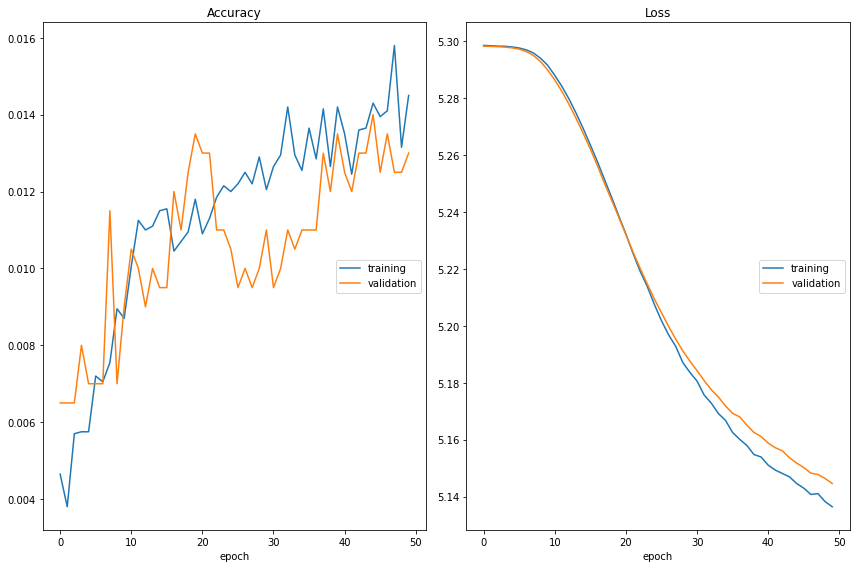
\includegraphics[width=\textwidth]{../figs/q2_acc.png}
		\caption{Network train and validation accuracy and loss logs along the epochs for the fine tunning task. (first experiment)}
		\label{img:q2_acc}
	\end{figure}
	\begin{figure}
		\centering
		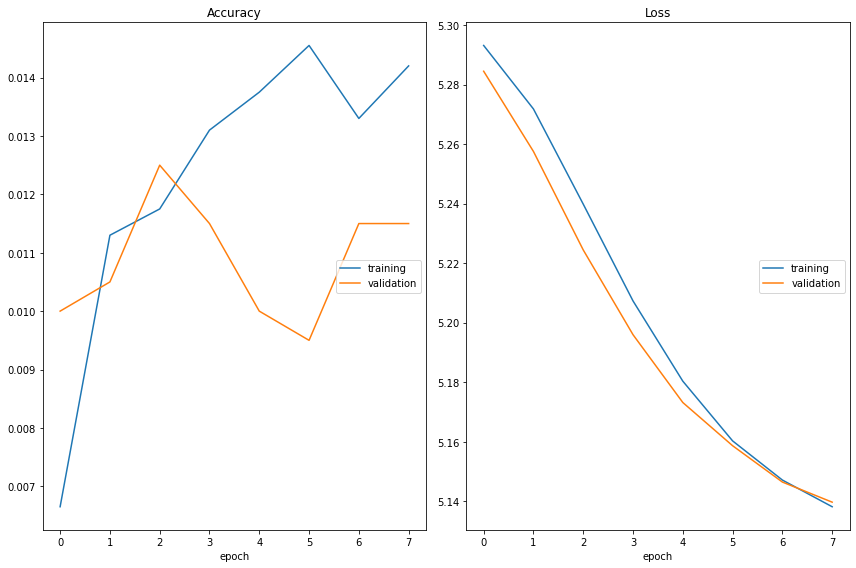
\includegraphics[width=\textwidth]{../figs/q2_acc_6.png}
		\caption{Network train and validation accuracy and loss logs along the epochs for the fine tuning task (second experiment).}
		\label{img:q2_acc_6}
	\end{figure}
	
	On the other hand, the third task shows a higher accuracy of \%26.4. It was expected that the accuracy for this model will be smaller than the accuracy achieved by the second task. As the second task is being fine-tuned on a very strong pre-trained model. To do the model ensemble classification, unfortunately, I was not able to complete the task because of receiving this error message: "NotImplementedError: Multilabel and multi-output classification is not supported." when I was trying to fit the model on training input and labels. And, unfortunately, I could not find a proper solution for that through the network and did not find more time to ask about it.
	\href{https://colab.research.google.com/drive/1LOb1nhmdRy_zXkRVinynlgsTIWOysq0U?authuser=1#scrollTo=7J7lbaO3QTNK\&line=1\&uniqifier=1}{Link for the third question}
	
	\begin{figure}
		\centering
		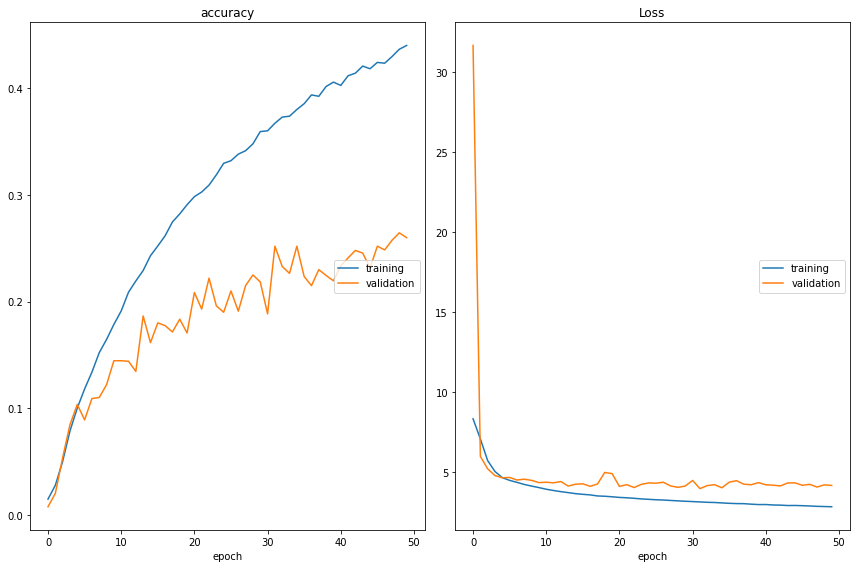
\includegraphics[width=\textwidth]{../figs/q3_acc.png}
		\caption{Network train and validation accuracy and loss logs along the epochs for the best model from assignment 2.}
		\label{img:q3_acc}
	\end{figure}
	
	
	\section{Conclusion}
	The point of this assignment was to be able to implement three different models: 1- just using a pre-trained model on a new dataset, 2- fine-tune the pre-trained model with the dataset, and 3- train the data on a DCNN model. Afterward, we could compare these three models together by ensembling the models. I expected to have a high accuracy in task 2 due to the power of pre-trained ResNet50 in addition to the time and effort spent to retrain the final layers. The two experiments done on the second task show that the result is not close to over-fitting as the training and validation accuracy and losses are too close to each other. Thus, having a much bigger iteration number may change the maximum accuracy significantly. Furthermore, the zero-padding method to increase the size of input images can be one of the sources of trouble. 
	As it can be seen there are different parameters responsible for choosing one of the three models such as the number of epochs, resize methods, the similarity between our dataset and the dataset that our model is trained with, also the size of the dataset can have an essential impact.
	
	%
	%\bibliography{bibfile} 
	%\bibliographystyle{ieeetr}
	
\end{document}